\documentclass[11pt,a4paper]{article}
\usepackage[utf8]{inputenc}
\usepackage[T1]{fontenc}
\usepackage[icelandic]{babel}
\usepackage{amsmath, amsthm, amssymb, amsfonts}

\usepackage{geometry}
\usepackage{hyperref}
\usepackage{fancyhdr}
\usepackage{graphicx}
\usepackage{color}
\usepackage[table]{xcolor}
\usepackage[ruled, vlined]{algorithm2e}
\usepackage{booktabs}
\usepackage{enumerate}
\usepackage{braket}
\usepackage[parfill]{parskip}
\usepackage{setspace}
\usepackage{tikz}
\usepackage{wrapfig}
\usepackage{dsfont}
\usepackage{subcaption}
 \usepackage{listings}
\lstset
{
	language=Python,
	basicstyle=\ttfamily\footnotesize,
	numbers=left,
	numberstyle=\small\color{gray},
	numbersep=5pt,
	showstringspaces=false,
	frame=single,
	tabsize=2,
	breaklines=true, 
	keywordstyle=\color{blue},
	commentstyle=\color{green},
	stringstyle=\color{red}, 
	escapeinside={\%*}{*)},
}
\geometry{includeheadfoot, margin=2.5cm}

\pagestyle{fancy}
\renewcommand{\headrulewidth}{0.3pt}
\renewcommand{\footrulewidth}{0.3pt}
\setlength{\headheight}{14pt}


\def\firstcircle{(90:1.2cm) circle (1.5cm)}
\def\secondcircle{(210:1.2cm) circle (1.5cm)}
\def\thirdcircle{(330:1.2cm) circle (1.5cm)}

\author{Róbert Karl Lárusson}

\lhead{Róbert Karl}\chead{}\rhead{Lattice Dynamics}
\lfoot{Professor: Sveinn Ólafsson \& Jón Tómas}\cfoot{\thepage}\rfoot{EÐL520M}

\begin{document}
\thispagestyle{empty}

\begin{doublespacing}
\begin{center} \huge\bf
University of Iceland \\	

\includegraphics[width=12cm]{HI-logo.jpg}\\
Solid State Physics \\
\emph{Fall  2014} \\ 
\vspace{1cm}
Numerical estimation of the energy spectrum and probability density of an electron in a periodic potential \\
\end{center}
\vspace{1cm}
\textit{Author: Róbert Karl Lárusson}
\end{doublespacing}
\newpage
\part*{Introduction and theory}
Our aim is to numerically estimate the energy spectrum of a atom for a specific \textbf{one dimensional} potential $V(x)$ with a period $a$. We will use \emph{Bloch waves} as the solutions $\psi_{nk}$ to the Shrödinger equation. Bloch waves are  a product of a plane wave $e^{ikx}$ and a periodic function $u_{nk}$ of same period $a$ (in this case representing the \emph{lattice constant}), meaning it has the property $u_{nk}(x)=u_{nk}(x+a)$. We will be representing $u_{nk}$ as a linear combination of planewaves,
\begin{align}
u_{nk} = \sum_{K^{\prime}} C_{kK^{\prime}} e^{-iK^{\prime}x} \label{unk}
\end{align}
taking the product of equation \ref{unk} and $e^{ikx}$ yields,
\begin{align}
\psi(x)_{n,k} = \sum_{K^{\prime}} C_{kK^{\prime}} e^{i(k-K^{\prime})x} \hspace{0.3cm} \text{where} \hspace{0.3cm} K^{\prime} = \frac{2\pi }{a}n^{\prime} \hspace{0.3cm} \text{where} \hspace{0.3cm} n^{\prime} \in \mathbb{Z}
\end{align}
The (one-dimensional) time-independant Shrödinger equation,
\begin{align}
E\psi(x) = -\frac{\hbar^2}{2m} \frac{d^2}{dx^2} \psi(x) + V(x) \psi(x) \hspace{0.5cm} \text{or} \hspace{0.5cm} E\psi(x) = \hat{H} \psi(x) \label{shr}
\end{align}
Where $\hat{H}$ is the Hamiltonian operator
\begin{align}
\hat{H} = -\frac{\hbar^2}{2m} \frac{d^2}{dx^2} + V(x) = \hat{H}_0 + V(x)
\end{align}
Thus in dirac notation, we can write the energy of the free particle ($V(x)=0$) as $E_{n,k}$
\begin{align}
\hat{H}_0 \ket{n,k} = E_{n,k} \ket{n,k} \hspace{0.5cm} \text{where} \hspace{0.5cm} E_{n,k} = \frac{\hbar^2}{2m^{*}}k^2
\end{align}
and let us represent equation \ref{shr} as the following eigenvalue problem,
\begin{align}
\hat{H} | n,k ) = \varepsilon_{n,k} |n,k) \label{ham}
\end{align}
To get $\hat{H}$'s energy spectrum, we take the inner product of equation \ref{ham} with $\ket{n,k-K}$ and get,
\begin{align}
\bra{n,k-K} \hat{H} | n,k) = \mathbf{HC}_k = \sum_{K^{\prime}} C_{kK^{\prime}} \left( E_{n,k-K^{\prime}} \delta_{KK^{\prime}} + \Braket{n,k-K|V|n,k-K^{\prime}} \right) = \varepsilon_k \mathbf{C}_k \label{hamil}
\end{align}
where $| n,k )$ and $\ket{n,k}$ are related by, $|n,k) = \sum_{K^{\prime}} C_{kK^{\prime}}\ket{n,k-K^{\prime}}$. From equation \ref{hamil} we start with,
\begin{align}
E_{n,k-K^{\prime}} \delta_{KK^{\prime}} = \frac{\hbar^2}{2m^{*}} (k-K^{\prime})^2 = \frac{\hbar^2}{2m^{*}} \left(k- \frac{2\pi }{a}n^{\prime} \right)^2 \delta_{KK^{\prime}} \label{first}
\end{align}
We will assume our potential is $V(x) = \pm \sin^2{\left( \frac{\pi x}{a}\right)}$ so the latter part of equation \ref{hamil} is,
\begin{align}
\Braket{n,k-K|V|n,k-K^{\prime}}  =  \int_0^a e^{-i(k-K^{\prime})x} V(x)  e^{i(k-K^{\prime})x} dx = \pm  \int_0^a V_0 \sin^2{\left(\frac{\pi x}{a}\right)} e^{i(K-K^{\prime})x} dx \label{latter}
\end{align}
We need dimensionless variables, looking at equations \ref{first} and \ref{latter}, we redefine the following, \\
\begin{align}
\frac{\hbar^2}{2m^{*}} \rightarrow 1 \hspace{1cm} a \rightarrow 1 \hspace{1cm} k^* \rightarrow \frac{2\pi}{a} k \hspace{1cm} x^* \rightarrow \frac{x}{a}
\end{align}
So, equation \ref{first} then becomes, 
\begin{align}
E_{n,k-K^{\prime}} \delta_{KK^{\prime}} = \left(k^*- n^{\prime} \right)^2 \delta_{KK^{\prime}} \label{diag}
\end{align}

And equation \ref{latter} becomes,
\begin{align}
\Braket{n,k-K|V|n,k-K^{\prime}}  =  \pm  V_0 \int_0^1  \sin^2{\left(\pi x^*\right)} e^{i(K-K^{\prime})x^*} dx \label{ints}
\end{align}
It's clear that the kinetic part of the energy is only non-zero at the diagonal elements of the matrix (where $K=K^{\prime}$). We write a Python script to numerically evaluate the integral in equation \ref{ints} and then we construct the Hamiltonian matrix, find its eigen- values \& vectors. We  use the eigenvalues to obtain a energy spectrum and the eigenvectors to calculate the eigenfunctions (equation \ref{unk}).
\section*{Results}

\begin{figure}[h]
        \centering
        \begin{subfigure}[h!]{0.5\textwidth}
                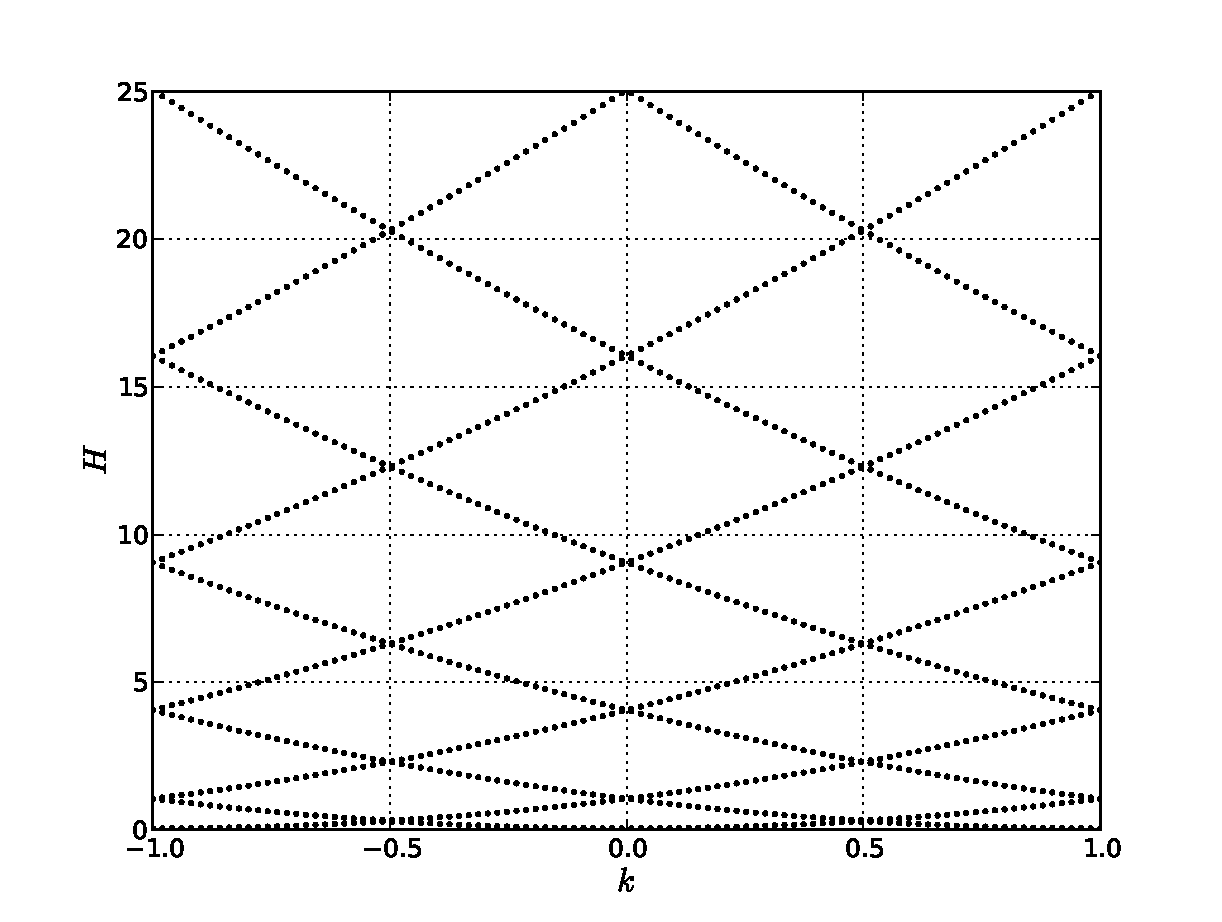
\includegraphics[width=\textwidth]{ener_spectrum/spectr_v01d10.pdf}
                \caption{The Energy spectrum for $V_0/E = 0.01$}
                \label{fig:1a}
        \end{subfigure}%
        ~ %add desired spacing between images, e. g. ~, \quad, \qquad etc.
          %(or a blank line to force the subfigure onto a new line)
        \begin{subfigure}[hb!]{0.5\textwidth}
                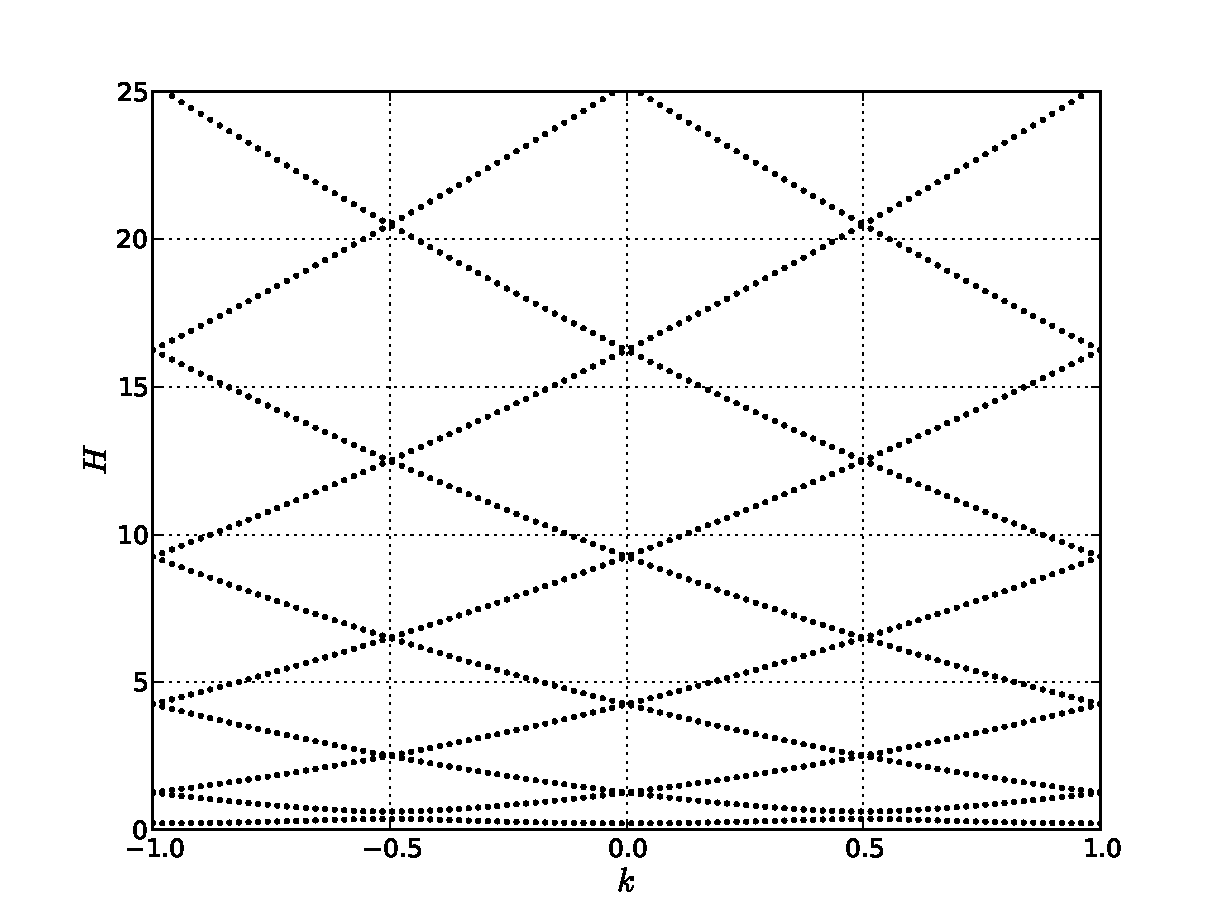
\includegraphics[width=\textwidth]{ener_spectrum/spectr_v01d2.pdf}
                \caption{$V_0/E = 0.5$}
                \label{fig:1b}
        \end{subfigure}
\caption{The energy spectrum for an electron in this periodic potential for two values of $V_0 < 1$}\label{fig:ener1}
\end{figure}

\begin{figure}[t]
\centering
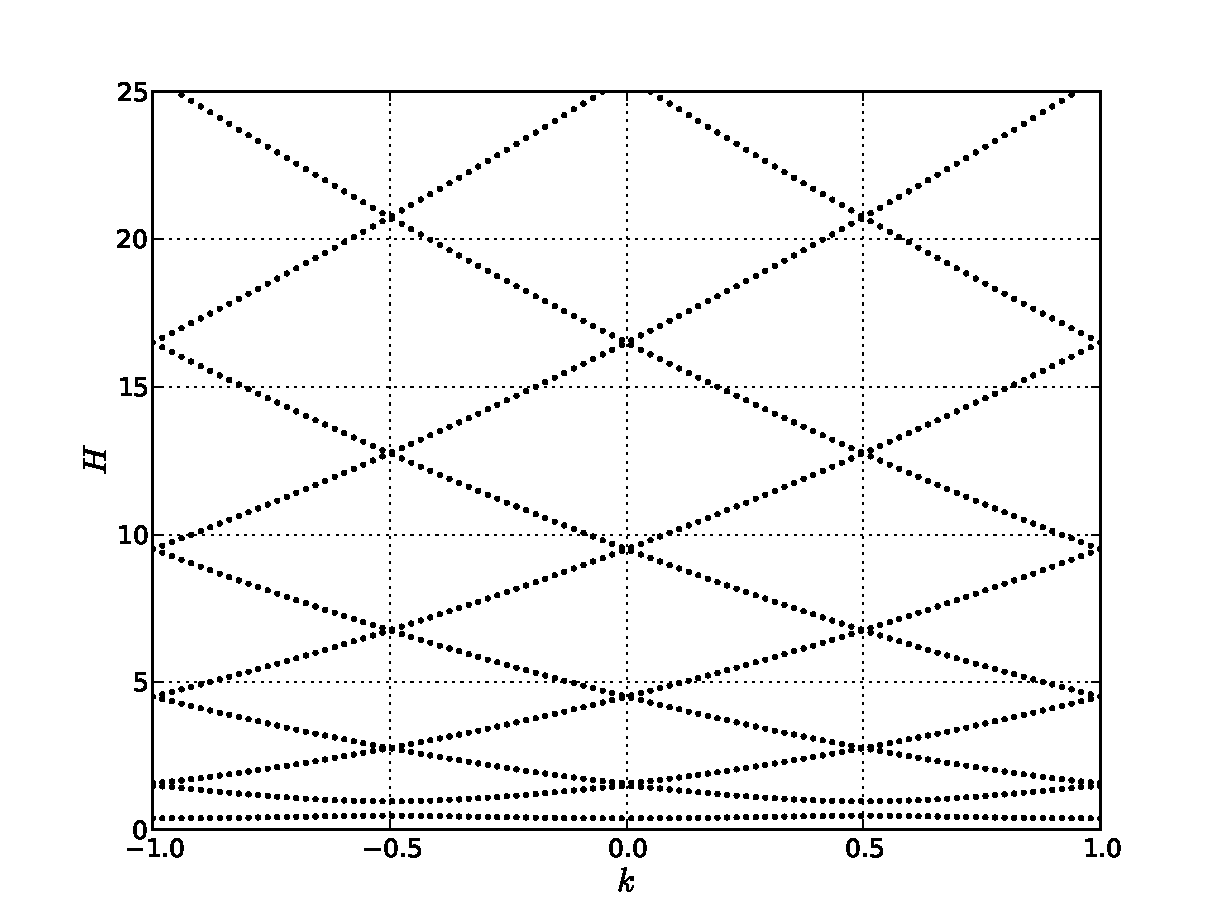
\includegraphics[width=0.9\textwidth]{ener_spectrum/spectr_v01.pdf}
\caption{Here we have the spectrum for $V_0/E=1$} \label{fig:ener2}
\end{figure}

\begin{figure}[hb!]
        \centering
        \begin{subfigure}[h!]{0.5\textwidth}
                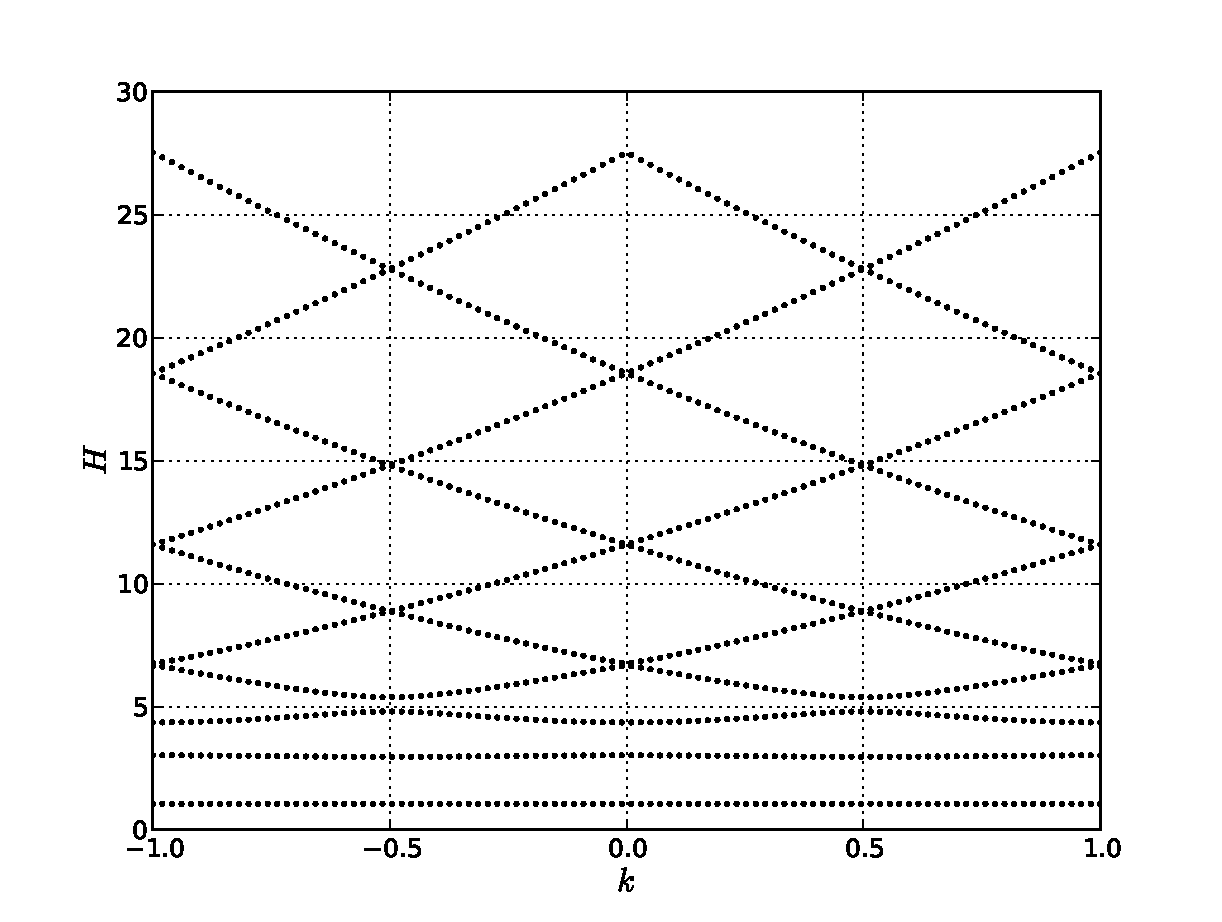
\includegraphics[width=\textwidth]{ener_spectrum/spectr_05tv01.pdf}
                \caption{The Energy spectrum for $V_0/E = 5.0$}
                \label{fig:3a}
        \end{subfigure}%
        ~ %add desired spacing between images, e. g. ~, \quad, \qquad etc.
          %(or a blank line to force the subfigure onto a new line)
        \begin{subfigure}[hb!]{0.5\textwidth}
                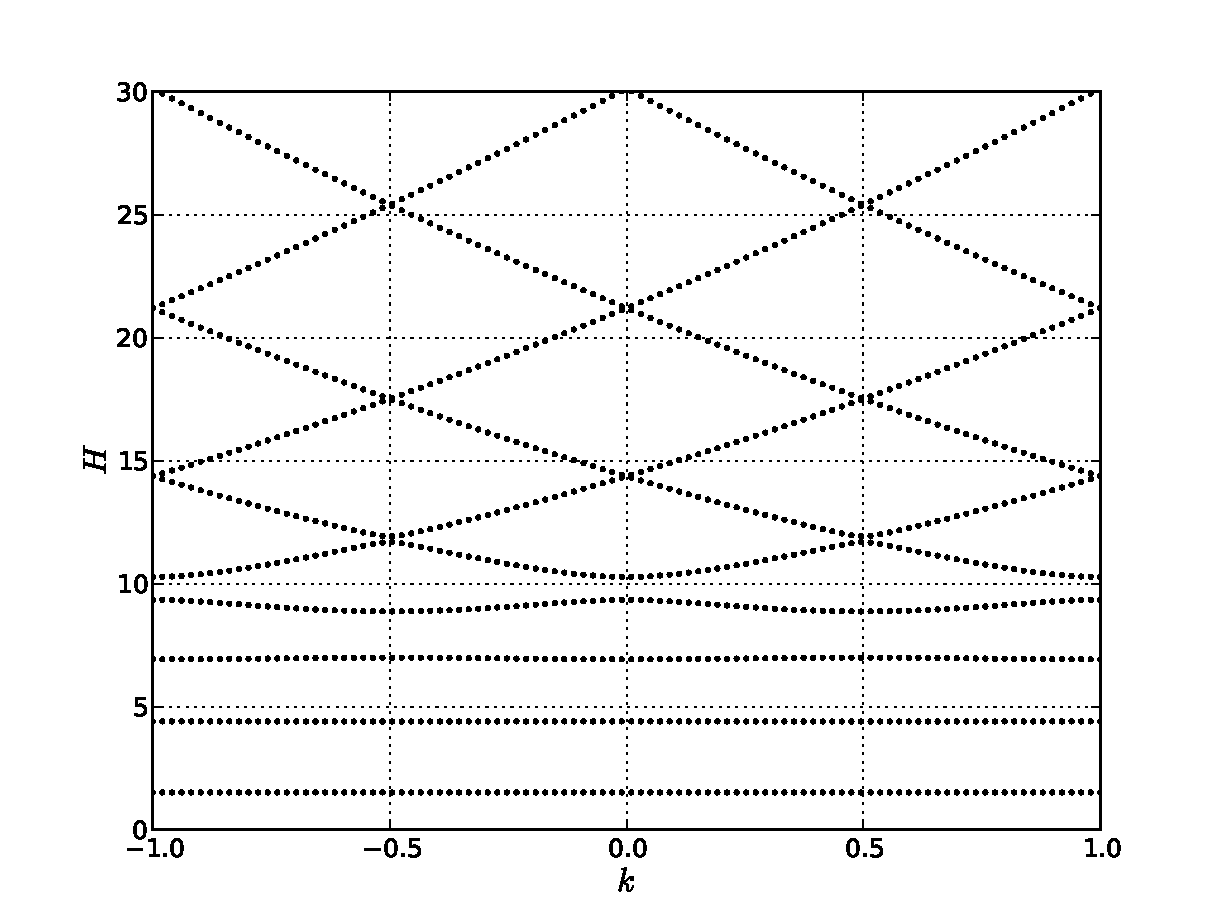
\includegraphics[width=\textwidth]{ener_spectrum/spectr_10tv01.pdf}
                \caption{$V_0/E = 10.0$}
                \label{fig:3b}
        \end{subfigure}
\caption{}\label{fig:ener3}
\end{figure}
From comparing figures \ref{fig:ener1} and \ref{fig:ener2} that the energy gap between levels increases as the potential $V_0$ increases.

\begin{figure}[t]
\centering
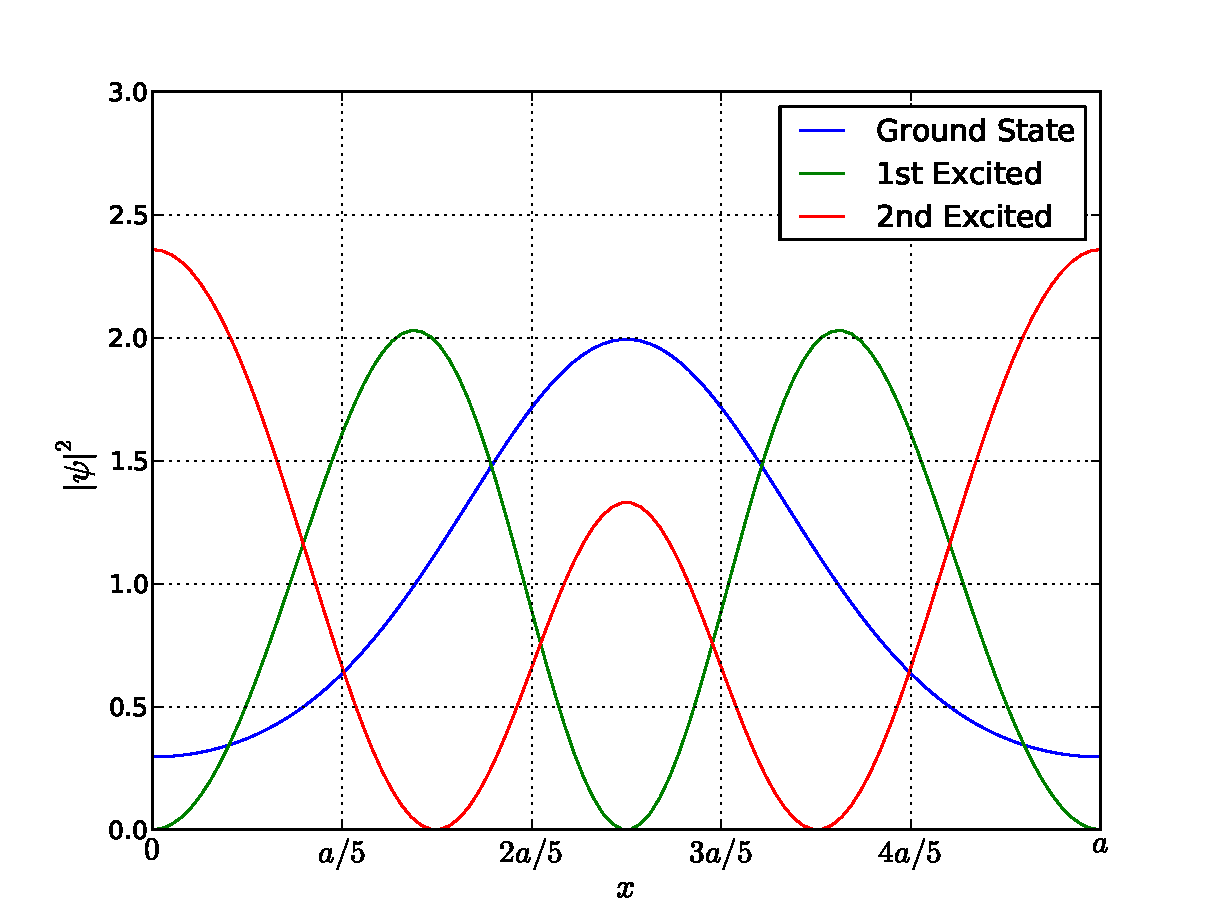
\includegraphics[width=0.9\textwidth]{prob_density/first3states.pdf}
\caption{The absolute value of the probability density squared for $V_0/E = 1.0$} \label{fig:psi1}
\end{figure}

\begin{figure}[hb!]
        \centering
        \begin{subfigure}[h!]{0.5\textwidth}
                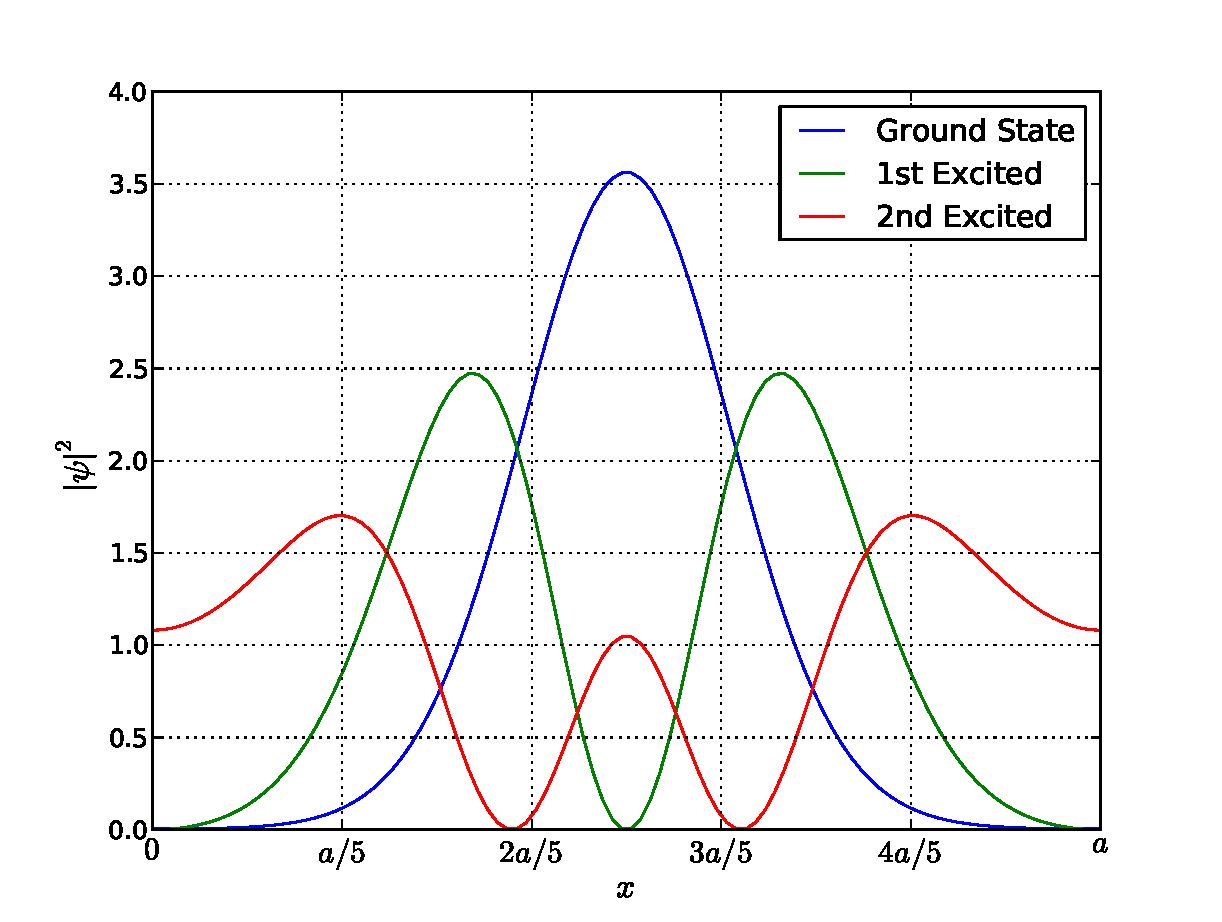
\includegraphics[width=\textwidth]{prob_density/first3states5tV.pdf}
                \caption{The Energy spectrum for $V_0/E = 5.0$}
                \label{fig:h4a}
        \end{subfigure}%
        ~ %add desired spacing between images, e. g. ~, \quad, \qquad etc.
          %(or a blank line to force the subfigure onto a new line)
        \begin{subfigure}[hb!]{0.5\textwidth}
                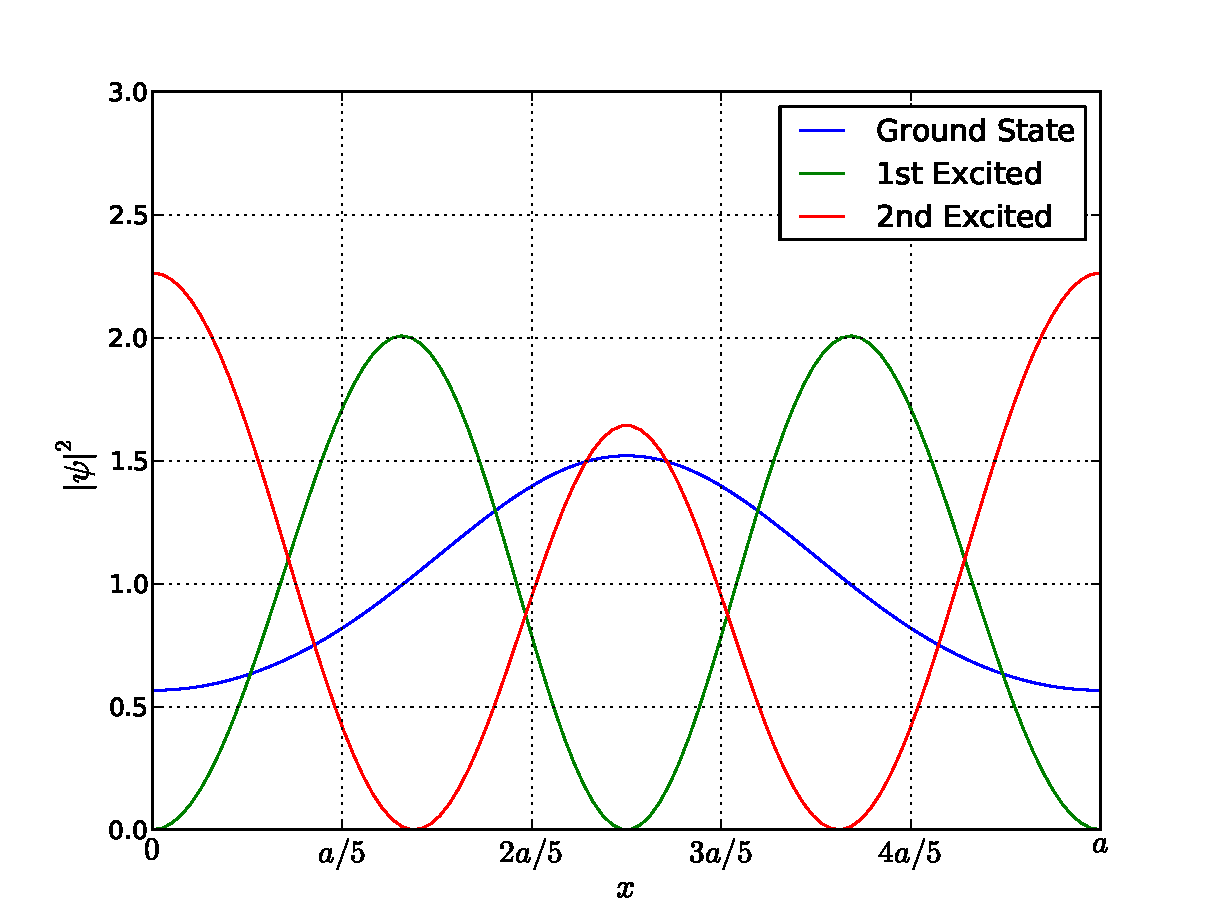
\includegraphics[width=\textwidth]{prob_density/first3statesVd2.pdf}
                \caption{$V_0/E = 0.5$}
                \label{fig:h4b}
        \end{subfigure}
\caption{Here we see the probabilty density for different values of $V_0$ }\label{fig:psi2}
\end{figure}

\clearpage
\section*{Source code}
\begin{lstlisting}
import numpy as np
from scipy.integrate import quad
from matplotlib import pyplot as plt

#DEFINE PARAMETERS
N = input('Pick the dimension of your basis, N = ')
V0 = input('Pick the amplitude of the periodic potential, V_0 = ') 
a = 1.0
kmaxDa=1.0
vidd = range(1,int(N+1)) #To map elements to array/matrix
stepsize=100

# FUNCTIONS THAT CALCULATES AN INTEGRAL AND STUFF
def integrFunc(x,k1,k2):  # integrFunc evaluates a function that we numerically evaluate.
    return (V0*(np.sin(np.pi*x)**2)*np.exp(complex(0,x*(k1-k2))).real)

def getEkin(k): # Returns expected kinetic energy (for a given value k (N values on a matrix diagonal))
    Ekin=[]
    for k2 in vidd:
        Ekin.append((2.0*np.pi*(k-(k2-N/2.0))**2))
    return np.diag(Ekin)

def getEpot(): # Returns the expected potential energy for a N by N basis
    Epot=[]
    for k2 in vidd:
        EpotCol=[]
        for k1 in vidd:
            EpotCol.append(-1*quad(integrFunc,0,a,args=(k1,k2))[0]) #Calculate the potential Energy 
        Epot.append(EpotCol)
    return Epot

def getHmat(k): # Returns a matrix representing the Hamiltonian (= getEkin + getEpot)
    Hmat=[]
    Kinetic = getEkin(k)
    for v in vidd:
        Hmat.append(map(sum, zip(Potential[v-1],Kinetic[v-1])))
    return Hmat

def getEigs(matrix): # Takes in a square matrix and returns its eigenvalues & eigenvectors.
    return np.linalg.eigh(matrix)

def getWavefunction(x,k,state): # Returns absolut value of the probabilty density squared for a given energystate, position x and wave vector k.
    probDens = 0.0
    for n in vidd:
        probDens = probDens + EigVec[n-1,state]*np.exp(complex(0,2.0*np.pi*(k-N/2.0-float(n))*x))
    return abs(probDens)**2

def makeMatrix(N): #Defines an array that contains N empty arrays.
    Fylki = []
    for incr in range(0,int(N)):
        Fylki.append([])
    return Fylki

Potential = getEpot()
kHnit = np.linspace(-kmaxDa,kmaxDa,stepsize)
yHnit = makeMatrix(N)
for k in kHnit:
    EigVal,EigVec = getEigs(getHmat(k))
    for g in vidd:
        yHnit[g-1].append(EigVal[g-1])

xHnit = np.linspace(0,1,stepsize)
states=range(0,3)
for state in states:
    psi=[]   
    for b in range(0,len(xHnit)):
        psi.append(getWavefunction(xHnit[b],100.0,state))
    plt.plot(xHnit,psi)
  
#CREATE & DEFINE THE PARAMETERS OF THE PLOT
for incr in range(0,5):
    plt.plot(kHnit,yHnit[incr],linestyle='', markersize=3,marker='o',color='black')                            #Create the plot
plt.ylabel('Energy $H_{nk}$',fontsize=16)                                     # Axis labels created
plt.xlabel('Wave number $k$',fontsize=16)
plt.ylim(0,35.0)
plt.xlim(-kmaxDa,kmaxDa)
plt.show()
\end{lstlisting}
\end{document}